\documentclass[a4paper, 11pt, titlepage, english]{article}

\usepackage{babel}
\usepackage[utf8]{inputenc}
\usepackage[T1]{fontenc, url}
\usepackage{textcomp}
\usepackage{amsmath, amssymb}
\usepackage{amsbsy, amsfonts}
\usepackage{graphicx, color}
\usepackage{parskip}
\usepackage{framed}
\usepackage{amsmath}
\usepackage{xcolor}
\usepackage{multicol}
\usepackage{url}
\usepackage{flafter}


\usepackage{geometry}
\geometry{headheight=0.01mm}
\geometry{top=24mm, bottom=30mm, left=39mm, right=39mm}

\definecolor{javared}{rgb}{0.6,0,0} % for strings
\definecolor{javagreen}{rgb}{0.25,0.5,0.35} % comments
\definecolor{javapurple}{rgb}{0.5,0,0.35} % keywords
\definecolor{javadocblue}{rgb}{0.25,0.35,0.75} % javadoc

\usepackage{listings}
\lstset{language=python,
basicstyle=\ttfamily\footnotesize,
keywordstyle=\color{javapurple}\bfseries,
stringstyle=\color{javared},
commentstyle=\color{javagreen},
morecomment=[s][\color{javadocblue}]{/**}{*/},
% numbers=left,
% numberstyle=\tiny\color{black},
stepnumber=2,
numbersep=10pt,
tabsize=2,
showspaces=false,
showstringspaces=false,
frame= single,
breaklines=true}

%
% Definering av egne kommandoer og miljøer
%
\newcommand{\dd}[1]{\ \text{d}#1}
\newcommand{\f}[2]{\frac{#1}{#2}} 
\newcommand{\beq}{\begin{equation*}}
\newcommand{\eeq}{\end{equation*}}
\newcommand{\bra}[1]{\langle #1|}
\newcommand{\ket}[1]{|#1 \rangle}
\newcommand{\braket}[2]{\langle #1 | #2 \rangle}
\newcommand{\braup}[1]{\langle #1 \left|\uparrow\rangle\right.}
\newcommand{\bradown}[1]{\langle #1 \left|\downarrow\rangle\right.}
\newcommand{\av}[1]{\left| #1 \right|}
\newcommand{\op}[1]{\hat{#1}}
\newcommand{\braopket}[3]{\langle #1 | {#2} | #3 \rangle}
\newcommand{\ketbra}[2]{\ket{#1}\bra{#2}}
\newcommand{\pp}[1]{\frac{\partial}{\partial #1}}
\newcommand{\ppn}[1]{\frac{\partial^2}{\partial #1^2}}
\newcommand{\up}{\left|\uparrow\rangle\right.}
\newcommand{\upup}{\left|\uparrow\uparrow\rangle\right.}
\newcommand{\down}{\left|\downarrow\rangle\right.}
\newcommand{\downdown}{\left|\downarrow\downarrow\rangle\right.}
\newcommand{\updown}{\left|\uparrow\downarrow\rangle\right.}
\newcommand{\downup}{\left|\downarrow\uparrow\rangle\right.}
\newcommand{\bupup}{\left.\langle\uparrow\uparrow\right|}
\newcommand{\bdowndown}{\left.\langle\downarrow\downarrow\right|}
\newcommand{\bupdown}{\left.\langle\uparrow\downarrow\right|}
\newcommand{\bdownup}{\left.\langle\downarrow\uparrow\right|}
\renewcommand{\d}{{\rm d}}

\newcommand{\To}{\quad \Rightarrow\quad}

\makeatletter
\renewcommand*\env@matrix[1][*\c@MaxMatrixCols c]{%
  \hskip -\arraycolsep
  \let\@ifnextchar\new@ifnextchar
  \array{#1}}
\makeatother

%
% navn og tittel
%
\author{Jonas van den Brink}
\title{Problem set 1 \\ FYS3140}


\begin{document}

\section*{Oppgave 1}
Vi antar at vi har stokastiske variable $X_1$, $X_2$, $\ldots$, $X_n$, som er er uavhengige og uniformt fordelt på intervallet $[0,\theta]$, dvs at de har tetthet
$$f(x; \theta) = \begin{cases}
                  1/\theta & \mbox{for } 0 \leq x \leq \theta, \\
                  0 & \mbox{ellers}.
                 \end{cases}$$
Parameteren $\theta$ er ukjent, og skal estimeres.
\subsection*{a)}
Vi starter med å finne forventingen av $X_i$, som per definisjon gitt ved
$$E(X_i) = \int_{-\infty}^\infty x f(x; \theta) \ \d x,$$
setter inn uttrykket for sannsynlighetsfordelingen og ser at bare $x\in(0,\theta]$ gir bidrag til integralet:
$$E(X_i) = \int_0^\theta \frac{x}{\theta} \ \d x = \frac{\theta^2}{2\theta} = \frac{\theta}{2}.$$

Vi kan finne variansen til $X_i$ fra uttrykket
$$V(X_i) = E(X_i^2) - E(X_i)^2,$$
vi må da først finne $E(X_i^2)$, som gjøres likt som tidligere:
$$E(X_i^2) = \int_{-\infty}^\infty x^2 f(x; \theta) \ \d x = \int_0^\theta \frac{x^2}{\theta} \ \d x = \frac{\theta^2}{3}.$$
Variansen er da
\begin{align*}
V(X_i) = E(X_i^2) - E(X_i)^2 = \frac{\theta^2}{12}.
\end{align*}

Vi har altså vist følgende
$$E(X_i) = \frac{\theta}{2}, \qquad V(X_i) = \frac{\theta^2}{12}.$$

\subsection*{b)}
Vi finner momentestimatoren for $\theta$ ved å sette det første distribusjonsmomentet, $E(X_i)$, lik det første samplingsmomentet, $\overline{X}$
$$E(X_i) = \frac{1}{n}\sum_{i=1}^n X_i,$$
vi setter inn for forventningen og løser for estimatoren
$$\frac{\hat{\theta}_{\rm mom}}{2} = \overline{X} \To \hat{\theta}_{\rm mom} = 2\overline{X}.$$

Forventningen av momentestimatoren blir
$$E(\hat{\theta}_{\rm mom}) = E(2\overline{X}),$$
setter inn for $\overline{X}$ og bruker linearitet av forventningen
\begin{align*}
E(\hat{\theta}_{\rm mom}) &= E\bigg(\frac{2}{n}\sum_{i=1}^n X_i\bigg) = \frac{2}{n}\sum_{i=1}^n E(X_i) = \frac{2}{n}\frac{n\theta}{2} =  \theta.
\end{align*}
Ettersom at 
$$E(\hat{\theta}_{\rm mom}) - \theta = 0,$$
ser vi at momentestimatoren er en forventningsrett estimator.

\subsection*{c)}
Standardfeilen til momentestimatoren er gitt ved
$$\sigma_{\hat{\theta}_{\rm mom}} = \sqrt{V(\hat{\theta}_{\rm mom})},$$
vi finner derfor først variansen til estimatoren, bruker da at vi generelt for variansen har
$$V\bigg(a + \sum_i b_i X_i\bigg) = \sum_i b_i^2 V(X_i).$$
Finner at
$$V(\hat{\theta}_{\rm mom}) = V\bigg(\sum_{i=1}^n \frac{2}{n} X_i\bigg) = \frac{4}{n^2}\sum_{i=1}^n V(X_i) = \frac{4}{n^2}\frac{n\theta^2}{12} = \frac{\theta^2}{3n}.$$
Slik at standardfeilen blir
$$\sigma_{\hat{\theta}_{\rm mom}} = \frac{\theta}{\sqrt{3n}}.$$

Vi kan nå vise at estimatoren er konsistent ved å bruke Chebychevs ulikhet, som sier at for enhver stokastisk variabel $X$, med forventning $\mu$ og varians $\sigma^2$, så vil
$$P(|X-\mu| > t) \leq \frac{\sigma^2}{t^2},$$
gjelde for alle $t > 0$. Momentestimatoren $\hat{\theta}_{\rm mom}$ er en stokastisk variabel med forventning $\mu=\theta$ og varians $\sigma^2 = \theta^2/3n$, vi setter dette inn i ulikheten og får
$$P(|\hat{\theta}_{\rm mom} - \theta| > t) \leq \frac{\theta^2}{3nt^2}.$$
Vi ser at for en hvilken $t > 0$ vi velger, kan vi gjøre uttrykket på høyre side mindre enn en hvilken som helst tolerans $\epsilon > 0$ ved å velge $n > N$ for en eller annen $N$. Det vil si at momentestimatoren konvergerer mot $\theta$ i sannsynlighet når $n$ vokser.

\subsection*{d)}
Siden de stokastiske variable $X_1$, $X_2$, $\ldots$ $X_n$ er uavhengige, så vil likelihooden være produktet av de individuelle sannsynlighetsfordelingene
$$f(x_1, x_2, \ldots, x_n; \theta) = \prod_{i=1}^n f(x_i; \theta).$$
Ved å sette inn $f(x_i; \theta)$ ser vi at produktet blir 
$$
f(x_1, x_2, \ldots, x_n; \theta) = \begin{cases}
                                      \big(1/\theta)^n & \mbox{ for } 0 \leq x_1, \ldots, x_n \leq \theta\\
                                      0 & \mbox { ellers.}
                                     \end{cases}.
$$

\subsection*{e)}
Vi skal nå finne maksimum likelihood estimatoren $\hat{\theta}_{\rm max}$, det vil si den verdien av den ukjente parameteren $\theta$ slik at likelihooden er maksimert: 
$$f(x_1, x_2, \ldots, x_n; \hat{\theta}_{\rm max}) \geq f(x_1, x_2, \ldots, x_n; \theta).$$ 
Vi er altså ute etter å finne et globalt maksimum i likelihood funksjon
$$
f(x_1, x_2, \ldots, x_n; \theta) = \begin{cases}
                                      \big(1/\theta)^n & \mbox{ for } 0 \leq x_1, \ldots, x_n \leq \theta\\
                                      0 & \mbox { ellers.}
                                     \end{cases}.
$$
Vi ser med en gang at en mindre $\theta$ betyr en større sannsynlighet, så lenge ikke $\theta < x_1, x_2, \ldots, x_n$, vi lar derfor 
$$\hat{\theta}_{\rm max} = \max_{1\leq i\leq n} X_i.$$
Merk at vi ikke kan finne dette maksimumet ved å derivere likelihood-funksjonen fordi likelihood funksjonen har en diskontinuitet akkurat i dette punktet.

\subsection*{f)}
Sannsynlighetstettheten til den største sampelen fra en stokastisk variabel med sannsynlighetstetthet $f(x)$ og kumulativ sannsynlighet $F(x)$  er gitt ved\footnote{Se \emph{Devore} \& \emph{Berk} avsnitt 5.5, side 268-269}
$$g_n(y) = n\big[F(y)\big]^{n-1} \cdot f(y).$$
Vi vet at for $X_i$ har vi tettheten
$$f(x; \theta) = \begin{cases}
                  1/\theta & \mbox{for } 0 \leq x \leq \theta, \\
                  0 & \mbox{ellers},
                 \end{cases}$$
slik at den kumulative sannsynligheten blir
$$F(x; \theta) = \begin{cases}
		  0 & \mbox{ for } x < 0 \\
		  \int_0^x  \frac{1}{\theta} \ \d x' = \frac{x}{\theta} & \mbox{ for } 0 \leq x \leq \theta \\
		  1 & \mbox{ for } x > \theta,
                 \end{cases}
                 $$
$$\int_0^x  \frac{1}{\theta} \ \d x' = \frac{x}{\theta}.$$
Innsetting gir da at sannsynlighetstettheten til maksimum likelihood estimatoren er
$$g_n(y) = n\bigg(\frac{y}{\theta}\bigg)^{n-1} \frac{1}{\theta} = \frac{ny^{n-1}}{\theta^n}.$$ 

\subsection*{g)}
Ettersom at vi nå kjenner sannsynlighetsfordelingen til maksimum likelihood estimatoren, kan vi finne forventningen til estimatoren direkte
$$E(\hat{\theta}_{\rm max}) = \int_{-\infty}^{\infty} y \cdot g_n(y) \ \d y,$$
innsetting gir
$$E(\hat{\theta}_{\rm max}) = \int_0^\theta \frac{nx^n}{\theta^n} \ \d y = \frac{n}{n+1}\theta.$$

\subsection*{h)}
Vi ser fra forventningen til maksimums likelihood estimatoren at den ikke er forventningsrett. Ettersom at forventningen er lineær, ser vi at vi kan lage en forventningsrett estimator ved å gange inn en faktor:
$$\hat{\theta}_{\rm mod} = \frac{n+1}{n}\hat{\theta}_{\rm max},$$
slik at vi har
$$E(\hat{\theta}_{\rm mod}) = E\bigg(\frac{n+1}{n}\hat{\theta}_{\rm max}\bigg) = \frac{n+1}{n} E(\hat{\theta}_{\rm max}) = \frac{n+1}{n}\frac{n}{n+1}\theta = \theta.$$

Standardfeilen til den modifiserte estimatoren blir
$$\sigma_{\hat{\theta}_{\rm mod}} = \sqrt{V(\hat{\theta}_{\rm mod})},$$
der variansen er
$$V(\hat{\theta}_{\rm mod}) = V\bigg(\frac{n+1}{n}\hat{\theta}_{\rm max}\bigg) = \frac{(n+1)^2}{n^2}V(\hat{\theta}_{\rm max}).$$
Variansen til maksimums likelihood estimatoren er igjen
$$V(\hat{\theta}_{\rm max}) = E(\hat{\theta}_{\rm max}^2) - E(\hat{\theta}_{\rm max})^2,$$
der 
$$E(\hat{\theta}_{\rm max}) = \frac{n}{n+1}\theta,$$
og 
$$E(\hat{\theta}_{\rm max}^2) = \int_0^\theta \frac{nx^{n+1}}{\theta^n} \ \d x = \frac{n}{n+2}\theta^2.$$

Innsetting gir da
$$V(\hat{\theta}_{\rm mod}) = \frac{(n+1)^2}{n^2} \bigg(\frac{n}{n+2}\theta^2 - \frac{n^2}{(n+1)^2}\theta^2\bigg),$$
som videre gir 
$$V(\hat{\theta}_{\rm mod}) = \frac{n^2+2n+1 - n^2 - 2n}{n(n+2)}\theta = \frac{\theta^2}{n(n+2)}.$$
Slik at standardfeilen er
$$\sigma_{\hat{\theta}_{\rm mod}} = \frac{\theta}{\sqrt{n(n+2)}}.$$

\subsection*{i)}
Vi har nå funnet to forventningsrette estimatorer:
$$\hat{\theta}_{\rm mom} = 2\overline{X}, \qquad \hat{\theta}_{\rm mod} = \frac{n+1}{n}\bigg(\max_{1\leq i\leq n} X_i\bigg).$$
Med standardfeilene
$$\sigma_{\hat{\theta}_{\rm mom}} = \frac{\theta}{\sqrt{3n}}, \qquad \sigma_{\hat{\theta}_{\rm mod}} = \frac{\theta}{\sqrt{n(n+2)}}.$$
Vi ser nå at selv om begge estimatorene konvergerer mot $\theta$ med økende $n$, så går momentestimatoren som $\mathcal{O}(1/\sqrt{n})$, mens den modifiserte estimatoren går som $\mathcal{O}(1/n)$. Den modifiserte estimatoren har altså en mye bedre asymptotisk oppførsel en momentestimatoren, om vi har mulighet til å ta mange samples er det altså den modifiserte estimatoren som er å foretrekke.

\subsection*{j)}
Vi skal nå gjennomføre et numerisk eksperiment for å teste resultatet vi har funnet. Vi trekker $n=20$ samples fra en uniform fordeling med parameter $\theta=1$, vi regner så ut hva de to estimatorene estimerer at $\theta$ faktisk er, vi gjør dette 1000 ganger på rad og lager et histogram av resultatene. For å undersøke den asymptotiske oppførselen til de to estimatoren gjentar vi forsøket for $n=200$ og $n=2000$. Se vedlegg 1 for kildekoden og figur \ref{fig:hist}, \ref{fig:hist2} og \ref{fig:hist3} for resultatene. 

Vi ser at den modifiserte estimatoren har en mye skarpere topp og ligger generelt sett nærmere den faktiske verdien av $\theta$ enn det momentestimatoren gjør, og vi ser at dette bare blir klarere når $n$ økes, slik som vi har kommet frem til. Vi ser også at momentestimatoren legger seg ganske symmetrisk om $\theta$, mens den modifiserte estimatoren derimot er asymmetrisk og har mer tendens til å legge seg under $\theta$.

\begin{figure}
\centering
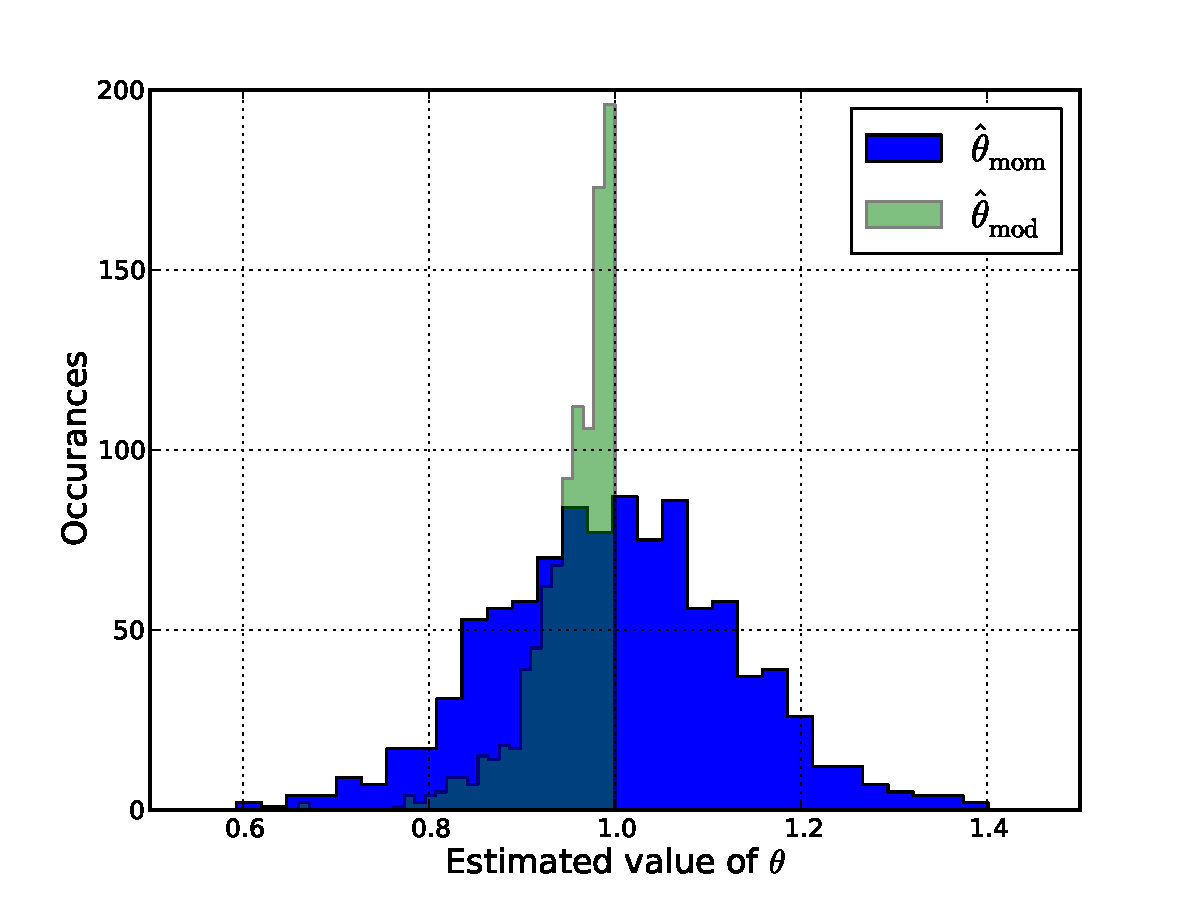
\includegraphics[width=\textwidth]{estimators_hist_n20.pdf}
\caption{Resultatene av $N=1000$ forsøk med $n=20$ samples hver presentert i et histogram. \label{fig:hist}}
\end{figure}

\begin{figure}
\centering
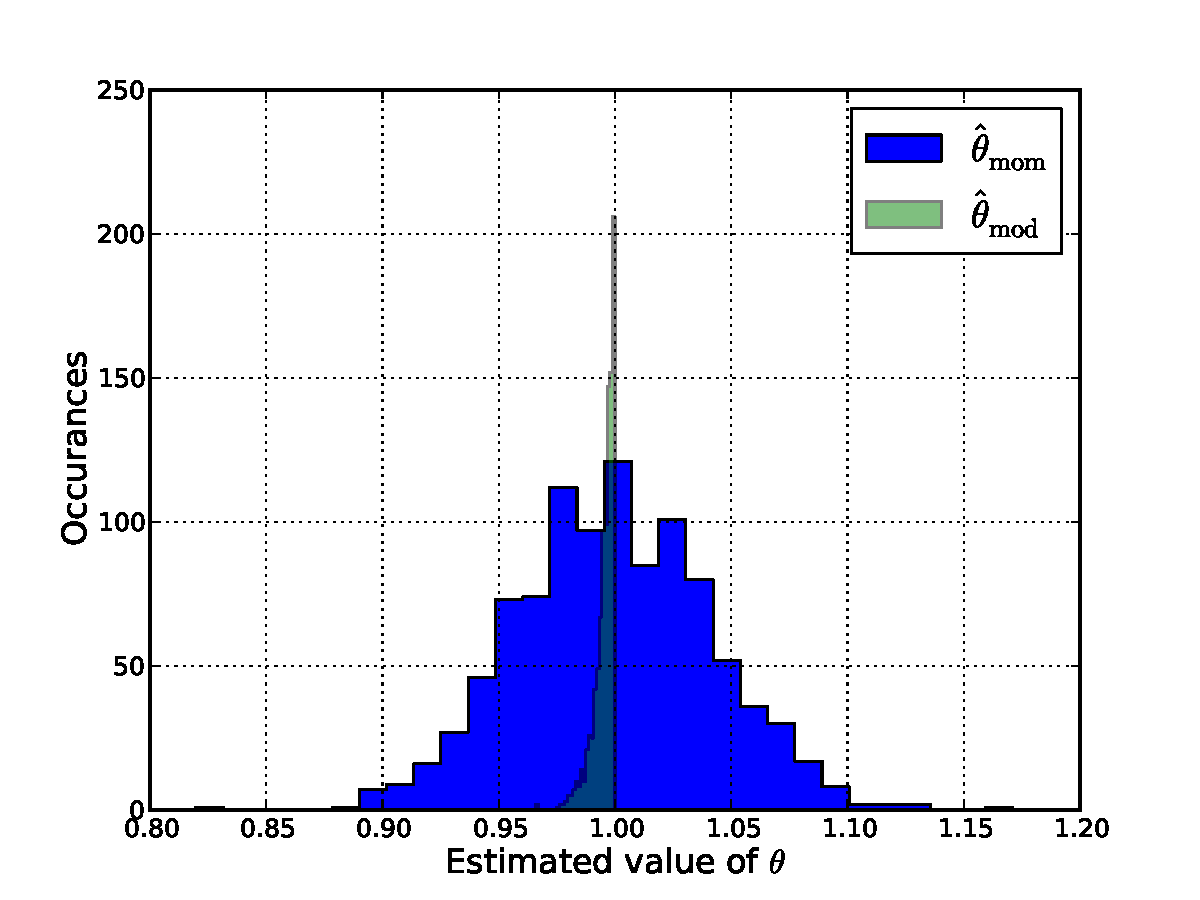
\includegraphics[width=\textwidth]{estimators_hist_n200.pdf}
\caption{Resultatene av $N=1000$ forsøk med $n=200$ samples hver presentert i et histogram. \label{fig:hist2}}
\end{figure}

\begin{figure}[t]
\centering
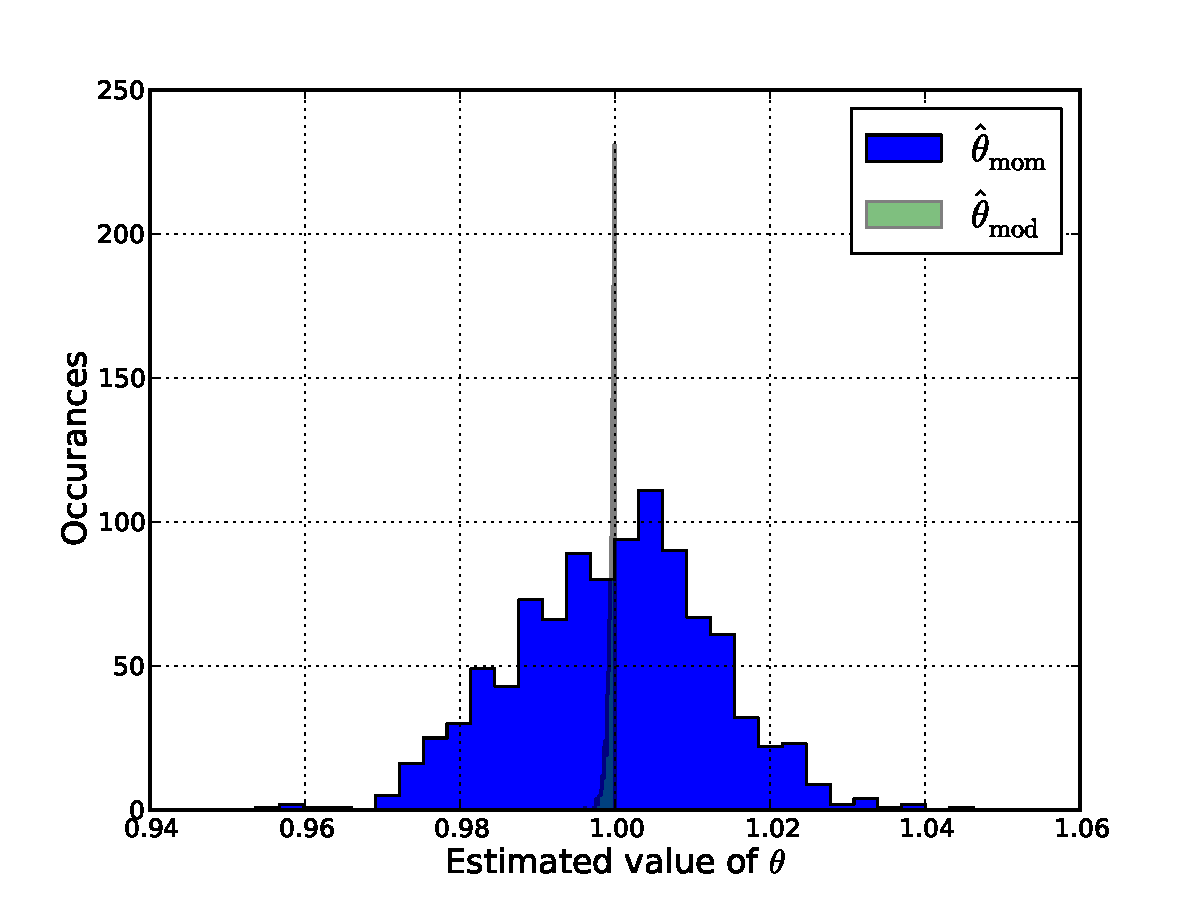
\includegraphics[width=\textwidth]{estimators_hist_n2000.pdf}
\caption{Resultatene av $N=1000$ forsøk med $n=2000$ samples hver presentert i et histogram. \label{fig:hist3}}
\end{figure}

\clearpage



\section*{Problem 2}
Ettersom at vi ikke kjenner det faktiske standardavviket $\sigma$, bruker vi istedet sample standardavviket $S$, vi finner derfor først $\overline{X}$ og $S$:
$$\overline{X} = 14.36, \quad S  = \sqrt{\frac{\sum_i (x_i - \overline{x})^2}{n-1}} = 1.156.$$
Et 95\% konfidensintervall for forventningen $\mu$ kan da finnes fra
$$P\bigg(-1.96 < \frac{\overline{X} - \mu}{S/\sqrt{n}}< 1.96 \bigg) \approx 0.95.$$
Vi manipulerer ulikheten og finner at
$$\overline{X} - \frac{1.96S}{\sqrt{n}} < \mu < \overline{X} + \frac{1.96S}{\sqrt{n}}.$$
Slik at konfidensintervallet er
$$\overline{X} \pm \frac{1.96S}{\sqrt{n}}.$$
Ved innsett av verdier finner vi at et 95\% konfidensintervall for $\mu$ er
$$(13.76, 14.97).$$


\clearpage

\section*{Vedlegg 1 - Kildekode til oppgave 1j}
\lstinputlisting{estimate.py}

\end{document}

